\documentclass[11pt]{article}
\usepackage{royden-report}
\usepackage[T1]{fontenc}
\usepackage{lmodern}
\usepackage{microtype,longtable,array,enumitem}
\setlist{itemsep=3pt,topsep=5pt}
\setcounter{tocdepth}{1}
\newcommand{\Dg}{\mathcal{D}}
\newcommand{\Ph}{\overline{\phi}}
\newcommand{\Zh}{\overline{\zeta}}
\newcommand{\Ps}{\overline{P}_1}
\newcommand{\Pt}{\overline{P}_2}
\newcommand{\papeq}[1]{\textup{Dysthe (#1)}}
\newcommand{\paperlink}[1]{\par\smallskip\noindent\textit{Return to the paper:} #1\par}
\newcommand{\checkpoint}[1]{\par\smallskip\noindent\textit{Readiness check.} #1\par}
\hypersetup{pdftitle={Before Reading Dysthe (1979): A Prerequisite Guide},pdfauthor={Prepared for Matas Vai}}
\title{Before Reading Dysthe (1979)\\\large A Prerequisite Guide to Deep-Water Wave Envelopes}
\author{}
\date{3 October 2026}
\begin{document}
\maketitle
\begin{abstract}
This guide assumes familiarity with partial differential equations and linear
algebra, but no previous course in water-wave theory or multiple-scale
perturbation methods. It develops the physical and mathematical background
needed to read K. B. Dysthe's 1979 paper, then works through its main stability
calculation. The emphasis is on why each approximation is made, what each
variable represents, and which conclusions the approximation supports.
\end{abstract}
\tableofcontents
\clearpage
\section{What you are preparing to understand}
\label{sec:orientation}

A nearly periodic surface wave can look regular while a small, long-scale
disturbance grows on top of it. Dysthe asks how well an approximate envelope
equation predicts that growth. The cubic nonlinear Schr\"odinger equation,
abbreviated NLS, is the leading model. He retains the next order in wave
steepness and finds that the current induced by a modulated wave changes
the prediction substantially \cite{dysthe}.

The paper is short because it assumes considerable background. Its hardest
steps are the choices of scales, harmonic components, and approximation order
that occur before the linear algebra begins. Your PDE background should make
Laplace's equation, Fourier modes, and the eigenvalue calculation familiar
once their physical roles are identified.

\subsection{A useful reading route}
Read Sections~\ref{sec:waves}--\ref{sec:asymptotics} first. They explain the
wave envelope, the moving free boundary, and why a slow derivative changes
the order of a term. Then study the NLS calculation in
Section~\ref{sec:nls} and the mean-flow calculation in
Section~\ref{sec:mean}. Finally, use
Sections~\ref{sec:dysthe}--\ref{sec:reading} beside the paper.
Appendix~\ref{sec:details} fills in two compressed derivative calculations.

You are ready for a first reading when you can explain
\begin{enumerate}
\item why the carrier oscillates rapidly but its envelope changes slowly;
\item why a deep-water Fourier mode decays exponentially below the surface;
\item why group velocity is half the phase velocity;
\item why a spatially varying intensity generates a mean current;
\item why a negative radicand in the stability formula means growth.
\end{enumerate}
For a derivation-level reading, also work through the determinant in
Section~\ref{sec:stability} and the order reduction in
Appendix~\ref{sec:details}. The exercises have answers.

\subsection{What is derived here and what is taken from the paper}
The linear water-wave dispersion relation, NLS perturbation calculation,
Fourier solution for the mean current, Dysthe stability determinant, and
small-steepness growth formulas are worked out here. The numerical
coefficients in the full fourth-order equation are transcribed from the
scanned paper. The guide explains the harmonic-expansion procedure that
produces them and the subsequent order reduction; it does not repeat
every nonlinear product in the intermediate quantity $Q$.

Agreement with Longuet-Higgins's full-equation calculations or laboratory
observations refers to \emph{comparisons reported in the 1979 paper}.
These are not new computations or independent validations. Our plots of
approximate formulas do not reproduce those reference data. Perturbative
derivations below are formal asymptotic calculations unless a proposition
explicitly states an exact result for a specified reduced model.

\subsection{Keep the different waves and frequencies separate}
The \emph{carrier} has dimensional wavenumber $k_0>0$ and linear angular
frequency $\omega_0=\sqrt{gk_0}$. The \emph{modulation} is a slower
variation of amplitude and phase. In the paper's dimensionless stability
calculation its wavenumbers are $\lambda,\mu$ and its frequency is $\Omega$.
Thus $\Omega$ is not $\omega_0$, and $\lambda$ is not the carrier wavelength.

\begin{longtable}{@{}p{.20\linewidth}p{.74\linewidth}@{}}
\toprule
Symbol & Meaning and convention\\
\midrule
\endhead
$x,y,z,t$ & Along-wave, transverse, vertical coordinates and time;
water lies below $z=\zeta$.\\
$g,\rho$ & Gravitational acceleration and constant water density.\\
$\zeta,\phi$ & Real surface elevation and real velocity potential;
fluid velocity is $\nabla\phi$.\\
$a,\varepsilon$ & Leading crest amplitude and steepness $\varepsilon=k_0a$;
wave height is approximately $2a$.\\
$\theta$ & Carrier phase $k_0x-\omega_0t$.\\
$A,B$ & Complex first-harmonic coefficients of potential and elevation.
They are different variables.\\
$\Ph,\Zh$ & Mean potential and mean elevation; the bar denotes a
carrier-period average.\\
$A^*,|A|^2$ & Complex conjugate and $AA^*$.\\
$A_0$ & Real dimensionless constant envelope amplitude; $A_0=k_0a$.\\
$a',\theta'$ & Small real amplitude and phase perturbations in (3.1);
primes here are not derivatives.\\
$\lambda,\mu,K$ & Dimensionless modulation wavenumbers in $x,y$ and
$K=\sqrt{\lambda^2+\mu^2}$.\\
$\Omega,\gamma$ & Modulation frequency and growth rate;
$\gamma=\operatorname{Im}\Omega$ for the growing mode.\\
$P_1,P_2;\ \Ps,\Pt$ & Differential operators in (3.2)--(3.3),
and algebraic quantities used in the dispersion relation.\\
\bottomrule
\end{longtable}

Coordinates are dimensional until Section~\ref{sec:scaling}, and thereafter
use Dysthe's dimensionless convention unless stated otherwise. Paper
equation numbers appear as \papeq{2.19}; other equation numbers refer to
this guide. Printed pages 105--114 correspond to PDF pages 2--11 because
the supplied file begins with a JSTOR cover page.
\clearpage

\section{From a surface wave to a complex envelope}
\label{sec:waves}
\subsection{Geometry, steepness, and deep water}
A linear plane wave travelling in the positive $x$ direction has elevation
\[
 \zeta(x,t)=a\cos(k_0x-\omega_0t).
\]
Its wavelength is $2\pi/k_0$, its period is $2\pi/\omega_0$, and its maximum
slope has magnitude $k_0a$. Steepness, rather than amplitude alone, measures
nonlinearity: a metre-high wave can be gentle at one wavelength and steep
at another.

\begin{assumption}[Physical setting]
The fluid is incompressible, inviscid, and irrotational, with constant
density; gravity supplies the restoring force. Surface tension, viscosity,
wind forcing, and wave breaking are excluded. The depth is treated as
infinite, the background is at rest, and $k_0a\ll1$.
\end{assumption}

At finite depth $h$, the carrier is in the deep-water regime when $k_0h\gg1$.
The infinite-depth idealization is stronger: a modulation-induced mean
response has depth scale $1/K_{\rm dim}$, often much larger than $1/k_0$.
A bottom negligible for the carrier need not be negligible for a very long
modulation. Dysthe uses an infinite lower half-space for both.

\subsection{Why use a complex variable for a real water surface?}
If $B=be^{i\beta}$, Euler's formula gives
\[
 Be^{i\theta}+B^*e^{-i\theta}=2b\cos(\theta+\beta).
\]
Magnitude and phase are stored together. A first harmonic written as
$Be^{i\theta}+\mathrm{c.c.}$ has crest amplitude $2|B|$, not $|B|$.
Here c.c. means to add the complex conjugate of the oscillatory terms;
a real mean component is included once.

A modulated surface is represented by
\begin{equation}\label{eq:surface-envelope}
 \zeta=\Zh+Be^{i\theta}+B^*e^{-i\theta}
       +\text{higher harmonics}.
\end{equation}
$B(x,y,t)$ changes little over one carrier wavelength or period. Its
magnitude controls local amplitude; its argument controls local phase.
Modulation includes changes in crest spacing and timing as well as height.

\begin{figure}[htbp]
\centering
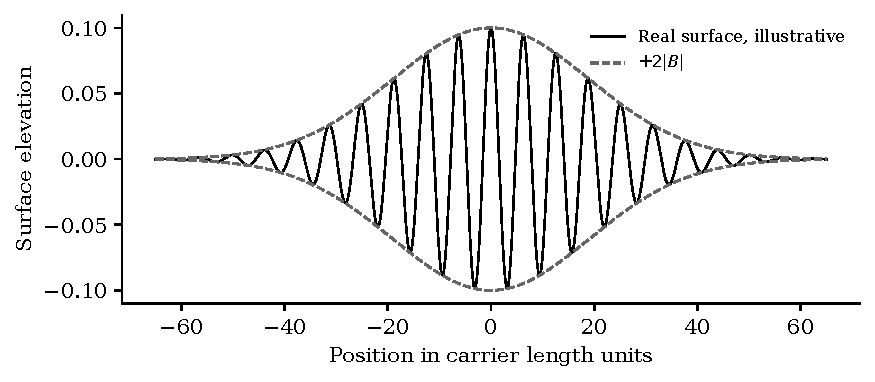
\includegraphics[width=\linewidth]{figures/carrier-envelope.pdf}
\caption{An illustrative carrier inside a slowly varying envelope at one
instant. Dashed curves are $\pm2|B|$. This is a schematic reconstruction,
not a computed Dysthe solution.}\label{fig:carrier}
\end{figure}

\subsection{Harmonics, sidebands, and the mean}
For a real narrowband wave there is a spectral cluster near $+k_0$ and a
conjugate cluster near $-k_0$. Narrowband means the width $\Delta k$ of
each cluster satisfies $\Delta k/k_0\ll1$.

A modulation creates \emph{sidebands} close to the carrier:
\[
 a[1+\delta\cos(qx)]\cos(k_0x)
 =a\cos(k_0x)+\frac{a\delta}{2}
   [\cos((k_0+q)x)+\cos((k_0-q)x)].
\]
These wavenumbers are near $k_0$ for $|q|\ll k_0$. A second
\emph{harmonic}, in contrast, has phase $2\theta$, near $2k_0$.
Nonlinear products generate harmonics even for a uniform wavetrain.
A \emph{mean} component has no fast carrier oscillation.

For $f=Be^{i\theta}+B^*e^{-i\theta}$,
\begin{equation}\label{eq:harmonic-product}
 f^2=B^2e^{2i\theta}+2|B|^2+(B^*)^2e^{-2i\theta}.
\end{equation}
A carrier-period average keeps $2|B|^2$ and removes the oscillatory terms.
A cubic product has first-harmonic coefficient $3|B|^2B$, explaining the
basic cubic structure of an envelope nonlinearity.

The average holds the slow coordinates effectively fixed. It is not an
average over the whole packet; its result can still vary in $x,y,t$.

\subsection{Potential envelope versus elevation envelope}
Dysthe writes the first-harmonic potential as
\[
 \phi=\Ph+A_{\rm dim}e^{k_0z}e^{i\theta}
 +A_{\rm dim}^*e^{k_0z}e^{-i\theta}+\cdots.
\]
The exponential describes depth decay. At leading linear order,
the dynamic surface condition gives
\begin{equation}\label{eq:AB}
 B_{\rm dim}=\frac{i\omega_0}{g}A_{\rm dim}.
\end{equation}
For a uniform carrier, $a=2|B_{\rm dim}|$. Hence the scaled potential
envelope in Dysthe (2.18) has
\[
 |A|=\frac{2k_0^2}{\omega_0}|A_{\rm dim}|=k_0a.
\]
Equal leading magnitudes do not make the envelopes interchangeable at fourth
order: their higher-order relations contain corrections.

\paperlink{Read (2.6), printed p.~107. Identify the carrier,
bound harmonics, and real mean fields.}
\checkpoint{Explain why $\mathrm{c.c.}$ makes the field real and
why the leading surface amplitude is $2|B|$.}
\clearpage

\section{The fluid problem behind the envelope equation}
\label{sec:fluid}
\subsection{Why Laplace's equation governs the fluid interior}
Let $\boldsymbol{u}=(u,v,w)$ denote velocity. Incompressibility is
$\nabla\cdot\boldsymbol{u}=0$; irrotationality is
$\nabla\times\boldsymbol{u}=0$. For a smooth flow in a simply connected
domain, the latter permits $\boldsymbol{u}=\nabla\phi$. Therefore
\begin{equation}\label{eq:laplace}
 \nabla^2\phi=0,\qquad z<\zeta(x,y,t).
\end{equation}
This is (2.1). It is a constraint at each time, not a wave equation in the
fluid interior. Time evolution enters through the surface conditions.

\subsection{Kinematic condition: the surface moves with the water}
Write the surface as $F=z-\zeta(x,y,t)=0$. A surface fluid particle must
remain there, so $DF/Dt=F_t+\boldsymbol{u}\cdot\nabla F=0$. Thus
\begin{equation}\label{eq:kinematic}
 \zeta_t+\phi_x\zeta_x+\phi_y\zeta_y=\phi_z,
 \qquad z=\zeta.
\end{equation}
The left side includes horizontal advection of a sloping surface.
$\zeta_t=\phi_z$ alone is the linearized condition.

\subsection{Dynamic condition: atmospheric pressure at the surface}
Integration of the inviscid potential-flow momentum equation gives
\[
 \phi_t+\frac12|\nabla\phi|^2+\frac p\rho+gz=C(t).
\]
An additive time-dependent change to $\phi$ absorbs $C(t)$. Subtract
constant atmospheric pressure and restrict to the surface:
\begin{equation}\label{eq:bernoulli}
 \phi_t+\frac12|\nabla\phi|^2+g\zeta=0,
 \qquad z=\zeta.
\end{equation}
This is Bernoulli's equation. Inviscid does not mean linear:
$|\nabla\phi|^2$ remains.

Dysthe's (2.2) differentiates Bernoulli along a surface fluid particle.
For smooth $f$, $Df/Dt=f_t+\nabla\phi\cdot\nabla f$.
Using the particle's vertical velocity $\phi_z$ gives
\begin{equation}\label{eq:dysthe-dynamic}
 \phi_{tt}+g\phi_z+\partial_t|\nabla\phi|^2
 +\frac12\nabla\phi\cdot\nabla|\nabla\phi|^2=0,
 \qquad z=\zeta.
\end{equation}
Differentiation of $\phi_t$ contributes
$\nabla\phi\cdot\nabla\phi_t$; differentiation of
$\tfrac12|\nabla\phi|^2$ contributes another equal term. Together they
give $\partial_t|\nabla\phi|^2$, explaining its coefficient in (2.2).

\subsection{Why expand the boundary condition about $z=0$?}
For smooth $f$ and small $\zeta$,
\begin{equation}\label{eq:boundary-taylor}
 f(x,y,\zeta,t)=f(x,y,0,t)+\zeta f_z(x,y,0,t)
 +\frac12\zeta^2 f_{zz}(x,y,0,t)+\cdots.
\end{equation}
This moves the equations to a fixed plane while retaining the effects of
surface displacement as extra terms. It does not flatten the actual wave.

In (2.4), $L=\partial_t^2+g\partial_z$. Taylor expansion of
\eqref{eq:dysthe-dynamic} gives
\[
 L\phi+\zeta L\phi_z+\partial_t|\nabla\phi|^2+Q=0,
 \qquad z=0,
\]
where the retained remainder is
\[
 Q=\frac12\zeta^2L\phi_{zz}
 +\frac12\nabla\phi\cdot\nabla|\nabla\phi|^2
 +\zeta\partial_{zt}|\nabla\phi|^2.
\]
These pieces come from another Taylor term, the cubic material derivative,
and the Taylor correction to the quadratic velocity term.

The expanded kinematic condition (2.5) is
\[
 \zeta_t-\phi_z+\nabla_h\cdot(\zeta\nabla_h\phi)
 +\nabla_h\cdot\left(\frac12\zeta^2\nabla_h\phi_z\right)=0,
 \qquad z=0,
\]
at the indicated order, where $\nabla_h=(\partial_x,\partial_y,0)$.
For example, its quadratic terms are initially
$\nabla_h\phi\cdot\nabla_h\zeta-\zeta\phi_{zz}$.
Since $-\phi_{zz}=\nabla_h^2\phi$, their sum becomes
$\nabla_h\cdot(\zeta\nabla_h\phi)$. The divergence form is an algebraic
reorganization, not an extra hypothesis.

\subsection{A first nonlinear calculation: the second Stokes harmonic}
A \emph{Stokes wavetrain} is a periodic travelling solution of the nonlinear
water-wave equations. Its surface is not exactly sinusoidal. Here is a short
calculation showing how a bound harmonic enters.

Suppress $y$ and let $\theta=k_0x-\omega_0t$, with
$\omega_0^2=gk_0$. The leading real potential is
\[
 \phi_1=\frac{a\omega_0}{k_0}e^{k_0z}\sin\theta.
\]
Through second order, try a bound elevation harmonic
$\zeta=a\cos\theta+C\cos(2\theta)$ and no second potential harmonic.
Expand Bernoulli at $z=0$. Its second-order part is
\[
 -ga^2k_0\cos^2\theta+\frac12a^2\omega_0^2
                         +gC\cos(2\theta)=0.
\]
Since $\cos^2\theta=(1+\cos2\theta)/2$, this gives
\begin{equation}\label{eq:stokes-second}
 C=\frac12k_0a^2,\qquad
 \zeta=a\cos\theta+\frac12k_0a^2\cos(2\theta)+\cdots.
\end{equation}
The kinematic condition independently gives
$2\omega_0C=k_0\omega_0a^2$, the same result. At a crest both elevation
terms are positive, while at a trough the second term is still positive;
the profile has sharper crests and flatter troughs. The harmonic oscillates
at $2\omega_0$, whereas a free linear mode of wavenumber $2k_0$ has
frequency $\sqrt2\omega_0$. It is therefore forced by the carrier,
not an independent linear wave. This simple calculation illustrates
the Stokes comparison mentioned immediately after (2.13).

\paperlink{Read (2.1)--(2.5), printed pp.~106--107.
Connect each equation to incompressibility, surface motion, or pressure.}
\checkpoint{Derive \eqref{eq:kinematic} from $DF/Dt=0$ and identify
which terms disappear upon linearization.}
\clearpage

\section{Linear deep-water waves and dispersion}
\label{sec:dispersion}
\subsection{Deriving the carrier dispersion relation}
Linearize about a flat, resting surface and evaluate at $z=0$:
\begin{equation}\label{eq:linear-bc}
 \zeta_t=\phi_z,\qquad \phi_t=-g\zeta.
\end{equation}
Take one complex Fourier component
\[
 \phi=Ce^{k_0z}e^{i(k_0x-\omega_0t)},\qquad
 \zeta=De^{i(k_0x-\omega_0t)}.
\]
Real fields include the conjugates. Laplace's equation holds because
$\partial_x^2$ contributes $-k_0^2$ and $\partial_z^2$ contributes $+k_0^2$.
$e^{k_0z}$ decays as $z\to-\infty$; the growing exponential is excluded.

The surface conditions give
\[
 -i\omega_0D=k_0C,\qquad -i\omega_0C=-gD.
\]
Elimination yields
\begin{equation}\label{eq:carrier-dispersion}
 \boxed{\omega_0^2=gk_0.}
\end{equation}
This also verifies \eqref{eq:AB}. For two horizontal directions, replace
$k_0$ by the horizontal wavevector's magnitude.

\subsection{Phase velocity and group velocity}
A crest has fixed phase $k_0x-\omega_0t$, so $c_p=\omega_0/k_0$.
To find packet velocity, add two nearby waves:
\begin{align*}
 &\cos((k_0+q)x-(\omega_0+\delta\omega)t)
 +\cos((k_0-q)x-(\omega_0-\delta\omega)t)\\
 &\hspace{1cm}=2\cos(qx-\delta\omega t)\cos(k_0x-\omega_0t).
\end{align*}
The slow factor travels at $\delta\omega/q$, tending to
$c_g=\omega'(k_0)$ in the narrowband limit. Thus
\begin{equation}\label{eq:group-speed}
 c_g=\frac{\omega_0}{2k_0}=\frac12c_p.
\end{equation}
Crests move through the group. The group is neither a particular crest nor
a collection of the same fluid particles.

$X=x-c_gt$ follows leading packet translation.
$\partial_t+c_g\partial_x$ measures evolution in that moving frame;
it is the transport derivative in (2.8).

\subsection{Dispersion curvature gives relative phase evolution}
For a nearby longitudinal wavenumber,
\[
 \omega(k_0+q)=\omega_0+c_gq+\tfrac12\omega''(k_0)q^2+\cdots,
 \qquad \omega''(k_0)=-\frac{\omega_0}{4k_0^2}.
\]
The constant is carrier frequency, the linear term gives translation, and
the quadratic term controls relative phase evolution within the packet.
In a PDE it is represented by a second derivative of the envelope.

Transverse curvature has the opposite sign. With dimensionless longitudinal
offset $q$ and transverse offset $r$,
\begin{equation}\label{eq:dispersion-series}
 \frac{\omega(k_0(1+q),k_0r)}{\omega_0}
 =1+\frac q2-\frac{q^2}{8}+\frac{r^2}{4}
 +\frac{q^3}{16}-\frac{3qr^2}{8}+O((|q|+|r|)^4).
\end{equation}
This explains the quadratic terms in NLS and the third derivatives in
Dysthe's equation. To check a PDE coefficient, insert
$e^{i(qx+ry-\nu t)}$ and compare its $\nu$ with this polynomial.

\begin{example}[A scale check]
For wavelength $10\,\mathrm{m}$, $k_0=2\pi/10\,\mathrm{m}^{-1}$.
Taking $g=9.81\,\mathrm{m\,s}^{-2}$ gives
$\omega_0\approx2.48\,\mathrm{s}^{-1}$,
$c_p\approx3.95\,\mathrm{m\,s}^{-1}$, and
$c_g\approx1.98\,\mathrm{m\,s}^{-1}$.
For $a=0.10\,\mathrm{m}$ the steepness is approximately $0.063$.
These are illustrative linear values, not breaking-wave predictions.
\end{example}

\subsection{What the deep-water limit removes}
For a flat bottom at $z=-h$, the no-normal-flow condition is
$\phi_z(-h)=0$. A linear horizontal mode then has vertical factor
$\cosh[k_0(z+h)]$ rather than $e^{k_0z}$. At the surface its logarithmic
vertical derivative is
\[
 \frac{\phi_z}{\phi}=k_0\tanh(k_0h).
\]
The same two linear surface conditions therefore give
\[
 \omega_0^2=gk_0\tanh(k_0h).
\]
For $k_0h\gg1$, $\tanh(k_0h)$ tends to one and
\eqref{eq:carrier-dispersion} is recovered. For $k_0h\ll1$,
$\tanh(k_0h)\approx k_0h$ and $\omega_0\approx k_0\sqrt{gh}$.
The shallow-water limiting phase and group speeds are equal; the deep-water
factor of two is a consequence of a different dispersion law.

This derivation explains why depth is a model assumption, not merely a
descriptive adjective. A change of depth modifies dispersion and the
mean-flow boundary problem, so one cannot retain the deep-water envelope
coefficients unchanged. Dysthe mentions finite-depth extensions in the
introduction, but the equations derived in this paper use infinite depth.

\paperlink{Read (2.7)--(2.8), p.~107, and the dispersive terms of (2.19),
p.~109. Optional reinforcement: \cite{plumb}.}
\checkpoint{Recover the $q^2$ and $r^2$ signs in
\eqref{eq:dispersion-series} from the expansion of $(1+s)^{1/4}$.}
\clearpage

\section{Weak nonlinearity and multiple-scale bookkeeping}
\label{sec:asymptotics}
\subsection{Two small quantities, with a chosen relationship}
Weak nonlinearity means $\varepsilon=k_0a\ll1$. Slow modulation means
$\delta=\Delta k/k_0\ll1$. They are distinct requirements. Dysthe balances
them by taking $\delta=O(\varepsilon)$. A small amplitude alone does not
make an arbitrary spectrum narrowband.

After choosing carrier units, display the scales as
\[
 X=\varepsilon(x-c_gt),\qquad Y=\varepsilon y,\qquad T=\varepsilon^2t.
\]
If $A=\varepsilon\alpha(X,Y,T)$, the chain rule gives
\begin{align*}
 A_x&=\varepsilon^2\alpha_X,& A_{xx}&=\varepsilon^3\alpha_{XX},\\
 A_t&=-c_g\varepsilon^2\alpha_X+\varepsilon^3\alpha_T,&
 (\partial_t+c_g\partial_x)A&=\varepsilon^3\alpha_T.
\end{align*}
The transport cancellation is essential: $A_t$ alone can be second order,
while the derivative following the group is third order.

\begin{definition}[Formal order]
Here $f=O(\varepsilon^m)$ means that the scaled coefficient of
$\varepsilon^m$ is treated as bounded in the chosen slow variables.
Products add orders. A derivative acting on a slow profile adds a factor
of $\varepsilon$, apart from the slower group-frame time scale.
\end{definition}
A rigorous bound would specify the domain, norm, derivative bounds, and
time interval, and prove uniform estimates. The paper's order statements
are formal bookkeeping, not an error theorem for arbitrary initial data.

\subsection{Distinguish slow derivatives from fast derivatives}
For the full oscillatory field,
\[
 \partial_x(Ae^{i\theta})=(A_x+ik_0A)e^{i\theta}.
\]
The carrier derivative $ik_0A$ does not raise the slow order. The statement
after (2.19) that a derivative adds an order concerns derivatives of the
slow coefficients. Carrier derivatives have already been extracted.

The vertical mean-flow scale is slow as well. Its depth dependence is
$e^{Kz}$ with $K=O(\varepsilon)$ in carrier units, whereas the carrier
has $e^z$ dependence.

\begin{center}
\begin{tabular}{@{}ll@{}}
\toprule Quantity in carrier units & Formal order\\\midrule
$A$ & $\varepsilon$\\
$A_x,A_y$ & $\varepsilon^2$\\
$\Dg A$, $\Dg=\partial_t+\tfrac12\partial_x$ & $\varepsilon^3$\\
$A_{xx},A_{yy},A|A|^2$ & $\varepsilon^3$\\
$A_{xxx},A_{xyy},|A|^2A_x,A^2A_x^*$ & $\varepsilon^4$\\
$\Ph$ & $\varepsilon^2$\\
$\Ph_x,\Ph_z,\Zh$ & $\varepsilon^3$\\
$A\Ph_x,A\Ph_z$ & $\varepsilon^4$\\\bottomrule
\end{tabular}
\end{center}

NLS keeps the third-order balance; Dysthe also keeps fourth-order terms.
``Fourth order'' refers to the perturbation expansion, not a fourth
spatial derivative or a quartic nonlinearity.

\subsection{Coefficient matching and resonance}
Insert the harmonic expansion into the boundary conditions. Collect the
coefficient of each $e^{im\theta}$ and the slow mean $m=0$ separately.
Higher harmonics are often determined by forced linear problems in terms
of $A$. They are \emph{bound}: their phase follows the carrier rather than
an independent linear frequency.

The fundamental $m=1$ is special. The leading linear operator already has
the carrier as a homogeneous solution; forcing at that phase can resonate.
The requirement that the next correction remain bounded supplies the
envelope evolution equation.

For comparison, $u_{tt}+u=\varepsilon\cos t$ has a particular term
$\tfrac12\varepsilon t\sin t$, which grows at long times. Allowing the
leading amplitude and phase to evolve slowly removes this secular forcing
from the next correction. This principle produces NLS and its next correction.

The cubic product in Section~\ref{sec:waves} explains the structure
$|A|^2A$ but not its water-wave coefficient. That coefficient comes from
the full boundary conditions, lower harmonics, and normalization.

\subsection{Order reduction}
An intermediate equation contains $A_{tt}$. Leading transport gives
$A_t\approx-\tfrac12A_x$, hence $A_{tt}\approx\tfrac14A_{xx}$.
For fourth-order accuracy one must also differentiate the third-order NLS
correction. Appendix~\ref{sec:reduction} shows this calculation.
Such substitutions are justified only when their errors lie beyond the
target order; they are not identities for arbitrary functions.

\paperlink{Read the order statements around (2.6), (2.12)--(2.17), and
after (2.19). Identify which derivatives act on slow coefficients.}
\checkpoint{For $A=\varepsilon\alpha(\varepsilon x)$, check that
$|A|^2A_x$ is fourth order and $|A|^2A$ third order.}
\clearpage

\section{NLS: the baseline approximation and its instability}
\label{sec:nls}
\subsection{Dysthe's dimensionless variables}
\label{sec:scaling}
From this point, use the transformation in (2.18). To make its meaning
unambiguous, write
\begin{align*}
 t&=\omega_0t_{\rm dim},& (x,y,z)&=k_0(x_{\rm dim},y_{\rm dim},z_{\rm dim}),\\
 A&=\frac{2k_0^2}{\omega_0}A_{\rm dim},&
 \Ph&=\frac{2k_0^2}{\omega_0}\Ph_{\rm dim},&
 \Zh&=k_0\Zh_{\rm dim}.
\end{align*}
The carrier phase becomes $x-t$ and $c_g=1/2$. These are carrier units,
not yet the separate slow coordinates $X,Y,T$. The envelope remains
$O(\varepsilon)$ and varies slowly in $x,y,t$.

Deleting the right side of (2.19) gives
\begin{equation}\label{eq:nls}
 2i\left(A_t+\frac12A_x\right)
 +\frac12A_{yy}-\frac14A_{xx}-|A|^2A=0.
\end{equation}
In the group coordinate $X=x-t/2$, a longitudinal envelope obeys
\[
 iA_t-\frac18A_{XX}-\frac12|A|^2A=0.
\]
Both coefficients are negative. Their product is positive, so this has
the focusing NLS sign combination; reversing time gives the frequently
used convention with two positive signs. A sign difference between
references need not imply different physics, but conventions must be checked.

The dispersive coefficients follow from \eqref{eq:dispersion-series}.
The cubic term describes an amplitude-dependent frequency shift. A
constant envelope solution is
\begin{equation}\label{eq:plane-wave}
 A=A_0e^{-iA_0^2t/2},\qquad A_0>0.
\end{equation}
Its magnitude is constant. Multiplication by the carrier gives total phase
$x-(1+A_0^2/2)t$ to this order. The extra phase rotation is the weakly
nonlinear Stokes frequency correction.

\subsection{What linear stability asks}
Stability asks whether a small disturbance of this particular solution
remains small initially or grows. It does not ask whether $|A|$ itself
oscillates, and it does not prove later breaking.

Introduce an independent small perturbation parameter $\eta$:
\begin{equation}\label{eq:perturbation}
 A=A_0[1+\eta u(x,y,t)]
       e^{i(\eta v(x,y,t)-A_0^2t/2)},
\end{equation}
where $u,v$ are real and $\eta\ll1$. To first order,
$A=A_0e^{-iA_0^2t/2}[1+\eta(u+iv)]+O(\eta^2)$.
The amplitude-expansion parameter $\varepsilon$ and perturbation parameter
$\eta$ have different jobs. Linearization discards $\eta^2$ while retaining
the prescribed powers of $A_0=O(\varepsilon)$.

Set $\Dg=\partial_t+\tfrac12\partial_x$ and
$P_2=\tfrac14\partial_y^2-\tfrac18\partial_x^2$.
Substituting \eqref{eq:perturbation} into \eqref{eq:nls}, cancelling the
background solution, and separating real and imaginary parts gives
\begin{equation}\label{eq:nls-linear}
 \Dg u+P_2v=0,\qquad
 \Dg v-P_2u+A_0^2u=0.
\end{equation}
One useful intermediate identity is
$|A|^2A=A_0^3e^{-iA_0^2t/2}[1+\eta(3u+iv)]+O(\eta^2)$.
The phase shift from the background cancels one part of this contribution.

\subsection{The Fourier-mode matrix calculation}
Use a complex representation for the perturbation modes and take real
parts at the end:
\[
 (u,v)=(\widehat u,\widehat v)e^{i(\lambda x+\mu y-\Omega t)}.
\]
Define
\[
 p=\frac{\lambda^2}{8}-\frac{\mu^2}{4},\qquad
 V=\Omega-\frac\lambda2.
\]
$\Dg$ acts as $-iV$ and $P_2$ acts as $p$. The homogeneous system is
\[
 \begin{pmatrix}-iV&p\\A_0^2-p&-iV\end{pmatrix}
 \begin{pmatrix}\widehat u\\\widehat v\end{pmatrix}=0.
\]
A nonzero perturbation requires determinant zero:
\begin{equation}\label{eq:nls-dispersion}
 \left(\Omega-\frac\lambda2\right)^2=p(p-A_0^2).
\end{equation}

\begin{proposition}[Growth in the linearized NLS model]
For $A_0>0$ and real $\lambda,\mu$, a growing Fourier mode exists precisely
when $0<p<A_0^2$. Its growth rate is
$\gamma=\sqrt{p(A_0^2-p)}$.
\end{proposition}
\begin{proof}
If $0<p<A_0^2$, the right side of \eqref{eq:nls-dispersion} is negative,
so one frequency has $\operatorname{Im}\Omega>0$. For
$\Omega=\Omega_r+i\gamma$, the time factor is
$e^{-i\Omega t}=e^{-i\Omega_rt}e^{\gamma t}$. Otherwise the roots are
real, including repeated roots at the boundaries, and have no positive
exponential growth rate.\qedhere
\end{proof}
Repeated boundary roots can require separate analysis of neutral or
algebraic behavior. The proposition concerns exponential mode growth only.

For longitudinal perturbations, $\mu=0$ and $p=\lambda^2/8$. Thus
\begin{equation}\label{eq:nls-results}
 0<|\lambda|<2\sqrt2 A_0,\qquad
 |\lambda_M|=2A_0,\qquad \gamma_M=\frac12A_0^2.
\end{equation}
To maximize growth, complete the square:
$p(A_0^2-p)=A_0^4/4-(p-A_0^2/2)^2$.
The fastest NLS disturbance therefore has $p=A_0^2/2$.

\subsection{Why transverse perturbations matter}
For two horizontal modulation directions, the maximum condition is
\begin{equation}\label{eq:hyperbola}
 \lambda^2-2\mu^2=4A_0^2.
\end{equation}
This hyperbola is unbounded. The NLS polynomial dispersion approximation
formally predicts equal maximum growth at arbitrarily large modulation
wavenumbers along it, although those wavenumbers violate the narrowband
assumption. Dysthe's correction reduces this degeneracy. It does not make
a small-bandwidth approximation valid at large bandwidth.

\paperlink{Read the introduction's discussion of NLS, then (3.1)--(3.7).
The matrix calculation above is the simpler version of Dysthe's calculation.}
\checkpoint{Explain why $\Omega$ with positive imaginary part grows for
the convention $e^{-i\Omega t}$.}
\clearpage

\section{The induced mean current: Dysthe's central new effect}
\label{sec:mean}
\subsection{Averaging reveals a response invisible in the carrier alone}
Quadratic wave quantities such as velocity products have a nonzero
carrier-period average. The wave therefore carries averaged momentum flux.
The wave contribution to that flux is called \emph{radiation stress}.
Here radiation means transport by waves, not electromagnetic radiation.
A uniform flux has no horizontal divergence; a spatially modulated flux
can exert an averaged force and generate a mean-flow response.

This is a physical interpretation. Dysthe determines the mean response
from the averaged potential-flow surface conditions, not by introducing
a separate viscous forcing law. The induced current remains irrotational
under the paper's hypotheses.

In dimensional variables his (2.9)--(2.11) read
\begin{align*}
 \Ph_t+g\Zh&=0,&&z=0,\\
 \Ph_z-\Zh_t&=\frac{2\omega_0}{g}\boldsymbol{k}_0\cdot
                   \nabla_h|A_{\rm dim}|^2,&&z=0,\\
 \nabla^2\Ph&=0,&&z<0.
\end{align*}
The dimensions of the forcing and of $\Ph_z$ are both velocity.
In carrier-scaled variables, these become
\begin{equation}\label{eq:mean-full}
 \Ph_t+2\Zh=0,\qquad
 \Ph_z-2\Zh_t=\partial_x|A|^2,\qquad
 \nabla^2\Ph=0.
\end{equation}
The first equation gives $\Zh=O(\varepsilon^3)$ because
$\Ph=O(\varepsilon^2)$ and its time derivative is slow.
Thus $\Zh_t=O(\varepsilon^4)$, whereas $\Ph_z$ and
$\partial_x|A|^2$ are third order. At the retained order,
\begin{equation}\label{eq:mean-bc}
 \Ph_z=\partial_x|A|^2\quad(z=0),\qquad
 \nabla^2\Ph=0\quad(z<0).
\end{equation}
Together with decay at depth and a choice of zero background current,
this determines the mean velocity. An additive potential constant is a
gauge freedom and has no physical velocity.

\subsection{Solve the boundary problem one Fourier mode at a time}
Let $I=|A|^2$, and suppose it has a Fourier component
$\widehat I e^{i(\lambda x+\mu y)}$ with
$K=\sqrt{\lambda^2+\mu^2}>0$. Seeking a decaying solution gives
\[
 \Ph=C e^{Kz}e^{i(\lambda x+\mu y)}.
\]
The surface condition is $KC=i\lambda\widehat I$, so
\begin{equation}\label{eq:mean-symbol}
 \widehat{\Ph}(0)=\frac{i\lambda}{K}\widehat I,
 \qquad
 \boxed{\widehat{\Ph_x}(0)=-\frac{\lambda^2}{K}\widehat I.}
\end{equation}
The horizontal current has a negative real Fourier multiplier. This is
exactly the source of the $\lambda^2/K$ term in the stability result.

At $K=0$, the forcing is zero. Set the derivative response to zero;
do not divide by $K$. A uniform wavetrain generates no mean-current
\emph{forcing in this model}. This does not mean that water under a
uniform Stokes wave has no particle drift. Eulerian induced mean flow and
Lagrangian Stokes drift are different quantities.

\subsection{Nonlocality and the Hilbert transform}
With no $y$ dependence, $K=|\lambda|$ and the current multiplier is
$-|\lambda|$. Define $|D_x|$ by the Fourier multiplier $|\lambda|$.
For the transform convention
\[
 \widehat f(\lambda)=\int_{\RR}f(x)e^{-i\lambda x}\,\rad x,
\]
the Hilbert transform $H$ has multiplier $-i\operatorname{sgn}\lambda$,
so $H\partial_x=|D_x|$. Consequently
\begin{equation}\label{eq:hilbert}
 \Ph_x(x,0)=-|D_x|I(x)=-H\partial_x I(x).
\end{equation}
This is nonlocal: knowing intensity at one point is not sufficient to
calculate the current there. One must solve the half-space problem, or
apply its Fourier multiplier to the full profile. Periodic profiles use
the corresponding discrete multiplier and zero mode.

\begin{example}[An explicitly solvable intensity modulation]
Let $I(x)=I_0+I_1\cos(\kappa x)$, where $\kappa>0$ and
$|I_1|<I_0$. Then
\[
 \Ph=-I_1e^{\kappa z}\sin(\kappa x),\qquad
 \Ph_x(x,0)=-\kappa I_1\cos(\kappa x).
\]
Differentiate to verify both Laplace's equation and
$\Ph_z=I_x$ at $z=0$. For $I_1>0$, the current response at an intensity
maximum is opposite the carrier propagation direction under this convention.
The response penetrates depth $1/\kappa$.
\end{example}

\begin{figure}[htbp]
\centering
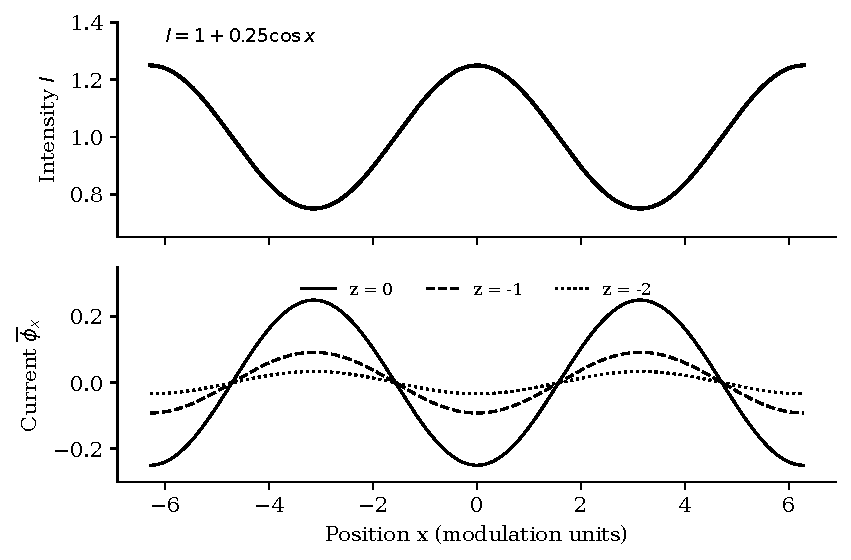
\includegraphics[width=.90\linewidth]{figures/mean-flow.pdf}
\caption{The cosine intensity example. The mean horizontal current
$\Ph_x$ is in opposite phase to the intensity variation, and its amplitude
decays as $e^{\kappa z}$. Vertical profiles use illustrative values;
the curves depict the analytic half-space solution.}\label{fig:mean}
\end{figure}

\subsection{Why a small current affects wave stability}
For a weak, slowly varying along-wave current $U$, the local dimensional
frequency has a Doppler contribution $k_0U$. In Dysthe's scaled envelope
equation the current is represented by $A\Ph_x$. Because the physical
scaling gives $k_0U/\omega_0=\Ph_x/2$, a locally uniform current produces
the expected envelope phase shift after the factor $2i$ is accounted for.

The intensity changes the current, the current changes local phase, and
phase changes feed back on the modulation. It is a coupled stability
mechanism. Calling it detuning does not imply that every disturbance is
stabilized or that the wave loses energy to viscosity.

\paperlink{Read (2.9)--(2.11), (2.20)--(2.21), and (4.1)--(4.3).
Then read the four physical steps on printed p.~114.}
\checkpoint{Derive the multiplier $-\lambda^2/K$ without using a
Hilbert-transform identity.}
\clearpage

\section{Reading the fourth-order envelope equation}
\label{sec:dysthe}
\subsection{The equation in the paper's convention}
At $z=0$, Dysthe (2.19) is
\begin{align}
 2i\left(A_t+\frac12A_x\right)
 +\frac12A_{yy}-\frac14A_{xx}-A|A|^2
 &= -\frac{i}{8}(6A_{xyy}-A_{xxx})\notag\\
 &\quad+\frac{3i}{2}A(AA_x^*-A^*A_x)
       +\frac i2|A|^2A_x\notag\\
 &\quad+A(\Ph_x-i\Ph_z).
 \label{eq:dysthe-full}
\end{align}
Subscripts denote partial derivatives and $A_x^*=\partial_x(A^*)$.
The mean field obeys \eqref{eq:mean-full}, or its consistently reduced
version \eqref{eq:mean-bc}. The right side is fourth order under
Section~\ref{sec:asymptotics}'s ordering. The left side is the NLS balance.

\begin{center}
\begin{tabular}{@{}p{.34\linewidth}p{.59\linewidth}@{}}
\toprule Term & Role\\\midrule
$2i(A_t+A_x/2)$ & Envelope change following the group.\\
$A_{yy}/2-A_{xx}/4$ & Leading transverse and longitudinal dispersion.\\
$-A|A|^2$ & Leading nonlinear phase shift.\\
$-i(6A_{xyy}-A_{xxx})/8$ & Next Taylor terms of linear dispersion.\\
$\tfrac{3i}{2}A(AA_x^*-A^*A_x)+\tfrac i2|A|^2A_x$
& Nonlinear effects involving envelope gradients.\\
$A(\Ph_x-i\Ph_z)$ & Coupling to the induced mean response.\\
\bottomrule
\end{tabular}
\end{center}

The combination $AA_x^*-A^*A_x$ is imaginary. If $A=Re^{i\psi}$ with
$R>0$, it equals $-2iR^2\psi_x$. Its role therefore involves a local phase
gradient. The term $\partial_x|A|^2$ instead measures amplitude variation.
These structures need not have the same effect even though both are slow.

\subsection{An algebraic evolution form of the printed equation}
Divide \eqref{eq:dysthe-full} by $2i$, move the right side to the left,
and use $\Ph_z=(|A|^2)_x$. At the retained order this gives
\begin{align}
 A_t+\frac12A_x+\frac i8A_{xx}-\frac i4A_{yy}
 +\frac i2|A|^2A
 &-\frac1{16}A_{xxx}+\frac38A_{xyy}\notag\\
 &+|A|^2A_x-\frac14A^2A_x^*
 +\frac i2A\Ph_x=0.
 \label{eq:dysthe-evolution}
\end{align}
The coefficient change in the gradient terms uses the vertical mean-flow
boundary condition. For example,
$\tfrac12A\Ph_z=\tfrac12|A|^2A_x+\tfrac12A^2A_x^*$.
This is why comparing partially reduced equations can make coefficients
appear inconsistent. Always record which mean-field terms have been eliminated.

For a longitudinal profile, \eqref{eq:hilbert} turns the last term into
$-\tfrac i2A|D_x|(|A|^2)$ in this temporal potential-envelope convention.
Other variables and spatial evolution conventions can have different signs
and coefficients. The original paper and the later spatial free-surface
model are compared separately in Appendix~\ref{sec:project}.

\subsection{A source-consistency issue to recognize}
\label{sec:source-consistency}
There is an apparent coefficient inconsistency in the supplied scan.
Taken literally, the printed plus sign in front of
$i|A|^2A_x/2$ in (2.19) gives the evolution form
\eqref{eq:dysthe-evolution}. Linearizing it gives
\[
 P_1u+\frac34A_0^2u_x+P_2v=0,\qquad
 P_1v+\frac54A_0^2v_x-P_2u+A_0^2u=-\frac12\Ph_x.
\]
In contrast, the paper's printed (3.2), after using
$\Ph_z=2A_0^2u_x$, has $5A_0^2u_x/4$; its (3.3) has
$7A_0^2v_x/4$. Changing the displayed $+i|A|^2A_x/2$ to a minus
would produce those two coefficients. This is an algebraic consistency
observation about the supplied scan; no publisher erratum has been verified.
The literal intermediate (2.17) also does not reproduce all the gradient
coefficients of (2.19); see Appendix~\ref{sec:reduction}.

For learning the main stability argument, the next section starts explicitly
from the printed linearized system (3.2)--(3.3), which does reproduce
(3.6)--(3.13). We preserve (2.19) as printed rather than silently editing
it. You should not conclude that a failure to match these particular
coefficients is a gap in your prerequisite knowledge. Nor should this guide
be used as an unqualified numerical implementation specification.

\subsection{What the simplified system in the conclusion means}
Dysthe (4.1)--(4.3) keeps just NLS and the horizontal current:
\begin{equation}\label{eq:simplified}
 2i\left(A_t+\frac12A_x\right)
 +\frac12A_{yy}-\frac14A_{xx}
 =A(|A|^2+\Ph_x),
\end{equation}
with \eqref{eq:mean-bc}. It captures the leading improvement in the
\emph{growth-rate and instability-band} calculations emphasized in the
paper. It is not an equality between complete fourth-order dynamics.

In particular, the full equation also shifts the real perturbation
frequency by terms containing $\lambda A_0^2$ and third powers of
modulation wavenumber. Those terms matter for phase or transport even
when they do not change the growth rate at the retained order. Calling
the mean current dominant is a statement about the particular stability
observables being studied, not about every possible wave-packet calculation.

\paperlink{Read (2.19), p.~109, using the table above. Compare it with
the explicitly simplified system on p.~113.}
\checkpoint{Derive \eqref{eq:dysthe-evolution} from the printed
\eqref{eq:dysthe-full}. Then compare its linearization with the
source-consistency note, rather than assuming every printed line agrees.}
\clearpage

\section{Working through Dysthe's stability calculation}
\label{sec:stability}
\subsection{Linearization about a uniform nonlinear wavetrain}
The uniform solution remains \eqref{eq:plane-wave}, with zero induced mean
current and elevation. Use \eqref{eq:perturbation}; Dysthe's $a',\theta'$
are our $\eta u,\eta v$. In this section the common factor $\eta$ is
suppressed, and the mean perturbation is first order in $\eta$.

Starting from the paper's printed equations (3.2)--(3.3), independently of
the discrepancy noted in Section~\ref{sec:source-consistency}, gives
\begin{align}
 P_1u+\frac14A_0^2u_x+P_2v&=-\frac12\Ph_z,
 \label{eq:dysthe-linear-a}\\
 P_1v+\frac74A_0^2v_x-P_2u+A_0^2u&=-\frac12\Ph_x,
 \label{eq:dysthe-linear-b}
\end{align}
where
\[
 P_1=\partial_t+\frac12\partial_x
 +\frac1{16}(6\partial_x\partial_y^2-\partial_x^3),
 \qquad P_2=\frac14\partial_y^2-\frac18\partial_x^2.
\]
The mean boundary condition linearizes as
\begin{equation}\label{eq:mean-linearized}
 \Ph_z=2A_0^2u_x,
\end{equation}
because $|A|^2=A_0^2(1+2\eta u)+O(\eta^2)$.

The extra $u_x$ term in \eqref{eq:dysthe-linear-a} changes from $1/4$ to
$5/4$ when its right side is moved left using \eqref{eq:mean-linearized}.

\subsection{Eliminate the mean field using the half-space solution}
For the mode $e^{i(\lambda x+\mu y-\Omega t)}$ with $K>0$,
\[
 \widehat{\Ph}(z)=\frac{2i\lambda A_0^2}{K}\widehat u\,e^{Kz},
 \qquad
 \widehat{\Ph_x}(0)=-\frac{2\lambda^2A_0^2}{K}\widehat u.
\]
Define the quantities used in the paper:
\begin{equation}\label{eq:Pbars}
 \Ps=\Omega-\frac\lambda2+\frac{\lambda}{16}(6\mu^2-\lambda^2),
 \qquad \Pt=\frac{\lambda^2}{8}-\frac{\mu^2}{4}.
\end{equation}
$P_1$ acts as $-i\Ps$, while $P_2$ acts as $\Pt$.
The bar in these two symbols is a paper convention for the algebraic
quantities, not a time average of the operators.

The two perturbation equations become
\begin{equation}\label{eq:dysthe-matrix}
 \begin{pmatrix}
 -i(\Ps-\frac54\lambda A_0^2)&\Pt\\
 A_0^2(1-\lambda^2/K)-\Pt&-i(\Ps-\frac74\lambda A_0^2)
 \end{pmatrix}
 \begin{pmatrix}\widehat u\\\widehat v\end{pmatrix}=0.
\end{equation}
Taking the determinant recovers (3.6):
\begin{equation}\label{eq:dysthe-det}
 (\Ps-\tfrac54\lambda A_0^2)(\Ps-\tfrac74\lambda A_0^2)
 =\Pt\{\Pt-A_0^2(1-\lambda^2/K)\}.
\end{equation}
The mean current modifies the effective nonlinear factor by
$1-\lambda^2/K$. Its dependence on modulation wavenumber is essential.

\subsection{Why the paper discards a term after solving the quadratic}
Completing the square gives the exact roots of this truncated determinant:
\begin{equation}\label{eq:exact-root-truncated}
 \Ps=\frac32\lambda A_0^2
 \mathbin{\pm}
 \sqrt{\Pt\{\Pt-A_0^2(1-\lambda^2/K)\}
              +\frac1{16}\lambda^2A_0^4}.
\end{equation}
But $A_0,\lambda,\mu=O(\varepsilon)$, so $\Pt=O(\varepsilon^2)$.
The radicand contains a leading fourth-order term and a fifth-order
mean-current correction. The added $\lambda^2A_0^4/16$ is sixth order.
Other contributions of that order could come from fifth-order terms
omitted from the original envelope equation. Retaining this one term
would not supply a consistently more accurate physical prediction.

Dysthe therefore uses the asymptotically consistent root (3.7):
\begin{equation}\label{eq:consistent-root}
 \Ps\simeq\frac32\lambda A_0^2
 \mathbin{\pm}\sqrt{\Pt\{\Pt-A_0^2(1-\lambda^2/K)\}}.
\end{equation}
Here $\simeq$ explicitly indicates truncation. Away from marginal roots,
the discarded sixth-order radicand term changes the frequency at fourth
order, beyond the third-order frequency correction supported by the
fourth-order field equation. Near a zero radicand, such square-root
expansions need extra care; do not claim a uniform error estimate there.

The real offset in \eqref{eq:Pbars} contains the higher linear dispersion;
$3\lambda A_0^2/2$ is also real. They shift mode frequency but do not
alter its imaginary part at this order. The growth-rate change is traced
to the horizontal induced current.

\subsection{Longitudinal instability band}
For $\mu=0$, $K=|\lambda|$, so the growing root has
\begin{equation}\label{eq:dysthe-growth}
 \gamma^2=\frac{\lambda^2}{8}
 \left[A_0^2(1-|\lambda|)-\frac{\lambda^2}{8}\right].
\end{equation}
Within the narrowband regime, the exponential instability condition is
\begin{equation}\label{eq:dysthe-band}
 0<\lambda^2<8A_0^2(1-|\lambda|).
\end{equation}
The explicit exclusion of $\lambda=0$ means that the uniform perturbation
has zero exponential growth. It is a neutral symmetry mode, not a growing
sideband.

For $\lambda>0$, solving the approximate marginal condition gives
\[
 \lambda_c=-4A_0^2+\sqrt{8A_0^2+16A_0^4}
           =2\sqrt2A_0-4A_0^2+O(A_0^3).
\]
This closed form is exact for the displayed approximate band equation,
not an all-orders water-wave stability boundary.

The real frequency from the full retained root is
\[
 \operatorname{Re}\Omega=\frac\lambda2+\frac{\lambda^3}{16}
                         +\frac32\lambda A_0^2
 \qquad(\mu=0,\ \gamma>0).
\]
At the marginal mode, retaining through $A_0^2$ gives
\begin{equation}\label{eq:marginal-frequency}
 \Omega_c\simeq\sqrt2A_0(1-\sqrt2A_0),
\end{equation}
which is Dysthe (3.9). Higher-order frequency terms require a
correspondingly higher-order determination of the cutoff.

\subsection{Find the fastest growing mode}
Set $s=A_0>0$ and use $\lambda>0$. Differentiate
\eqref{eq:dysthe-growth}:
\[
 \gamma^2=\frac{s^2\lambda^2}{8}
          -\frac{s^2\lambda^3}{8}-\frac{\lambda^4}{64},
 \qquad
 \frac{\rad\gamma^2}{\rad\lambda}
 =\frac\lambda{16}(4s^2-6s^2\lambda-\lambda^2).
\]
The positive stationary root is
$\lambda_M=-3s^2+\sqrt{4s^2+9s^4}$. Expand at small $s$:
\begin{equation}\label{eq:lambda-max}
 \lambda_M=2s-3s^2+O(s^3).
\end{equation}
Substitution into the growth formula gives
$\gamma_M^2=s^4/4-s^5+O(s^6)$ and hence
\begin{equation}\label{eq:gamma-max}
 \gamma_M=\frac12s^2(1-2s)+O(s^4).
\end{equation}
Finally, substituting \eqref{eq:lambda-max} into the real frequency and
retaining through $s^2$ gives
\begin{equation}\label{eq:frequency-max}
 \operatorname{Re}\Omega_M=s(1-\tfrac32s)+O(s^3).
\end{equation}
These are (3.10)--(3.12). The mode and maximum-growth corrections have
different absolute orders because the leading quantities have different
orders. The approximate formula at $s=0.5$ must not be interpreted as an
established complete stabilization threshold.

\begin{figure}[htbp]
\centering
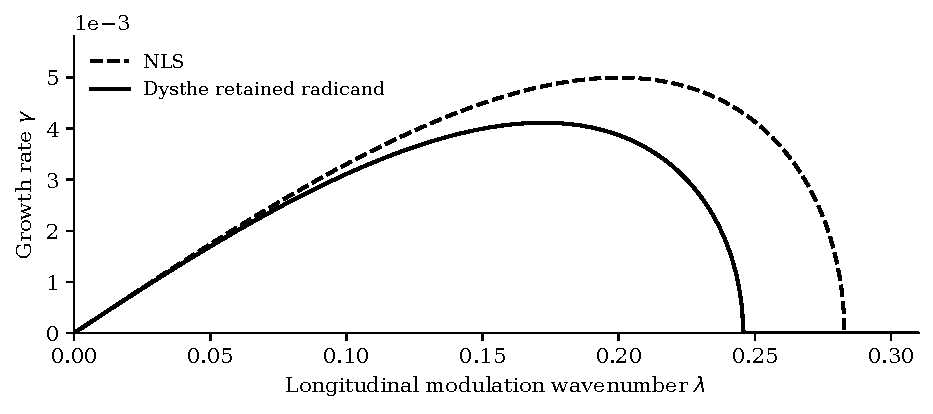
\includegraphics[width=\linewidth]{figures/longitudinal-growth.pdf}
\caption{Growth rates from the NLS radicand and Dysthe's consistently
truncated radicand, for illustrative $A_0=0.10$. These curves compare
reduced formulas; no full-equation or experimental data are included.}
\label{fig:growth}
\end{figure}

\subsection{Transverse modulations and the paper's figures}
For general $\lambda,\mu$, the retained growing root is
\begin{equation}\label{eq:oblique-growth}
 \gamma=\sqrt{[A_0^2(1-\lambda^2/K)-\Pt]\Pt},
\end{equation}
where the radicand must be positive and the wavevector must lie in the
slow-modulation regime. For small $K$, the effective nonlinear factor is
positive, so instability requires
$0<\Pt<A_0^2(1-\lambda^2/K)$.
The current correction depends on the direction of the modulation as
well as its size. Dysthe finds the largest retained growth for $\mu=0$,
removing the unbounded maximum-growth hyperbola of NLS.

The paper also discusses a formal large-$K$ cutoff near $3/2$, and
explicitly notes that this is outside the model's validity range.
Do not turn that formal feature into a physical cutoff theorem.

\begin{figure}[htbp]
\centering
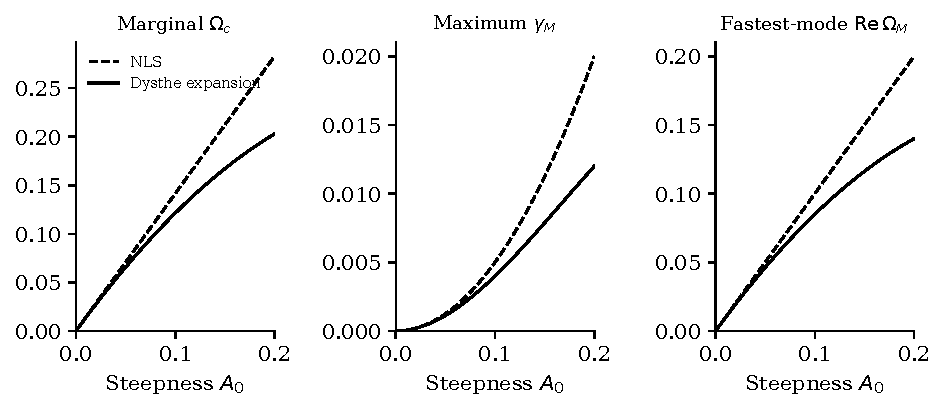
\includegraphics[width=\linewidth]{figures/asymptotic-comparison.pdf}
\caption{The leading NLS formulas and the small-steepness corrections
(3.9), (3.10), and (3.12), plotted only to $A_0=0.20$ for illustration.
The full-equation and laboratory curves in Dysthe's original figures are
not reproduced.}\label{fig:comparison}
\end{figure}

Read the original figures as follows. Figure~1 plots the modulation
frequency at marginal stability, not the carrier frequency.
Figure~2 plots the maximum exponential growth rate.
Figure~3 plots the real frequency separation of the fastest growing
sideband, not its growth rate. The paper reports especially good
agreement of (3.9)--(3.10) with its reference calculations below steepness
roughly $0.3$, while (3.12) underestimates the frequency shift above roughly
$0.2$. These are observable-specific comparisons, not a guarantee of
accuracy for every packet throughout that range.

\paperlink{Read (3.1)--(3.13), printed pp.~110--113. Follow
\eqref{eq:dysthe-matrix} to \eqref{eq:consistent-root}, then compare each
of the three original figure axes with the corresponding formula.}
\checkpoint{Complete the square in \eqref{eq:dysthe-det} and explain
why its exact algebraic root is not a higher-order physical result.}
\clearpage

\section{The long-wave check and a map back to the paper}
\label{sec:reading}
\subsection{Why Whitham theory appears near the end}
The paper uses a second approximation method as a consistency check.
Whitham modulation theory describes a locally periodic nonlinear wave
whose parameters change on scales much longer than its period and
wavelength. NLS assumes small amplitude and a narrow band. Whitham's
approach need not start with a small-amplitude carrier, but its modulation
must be very long. These are overlapping, rather than identical, assumptions.

For a longitudinal perturbation with $\lambda>0$ tending to zero,
\eqref{eq:consistent-root} gives
\begin{equation}\label{eq:long-wave}
 \Omega\simeq\frac\lambda2+\frac32\lambda A_0^2
              \mathbin{\pm}i\frac{\lambda A_0}{2\sqrt2}.
\end{equation}
The $\lambda^3$ linear-dispersion correction vanishes in this limit, and
$\lambda^2/K=|\lambda|$ tends to zero. The real correction proportional
to $\lambda A_0^2$ survives. This is the stated long-wave result (3.14).
For negative $\lambda$, the growing branch uses $|\lambda|$ in its
positive growth rate.

\subsection{Averaged Lagrangian: the minimum needed for (3.15)}
A Lagrangian is a function whose variation produces evolution equations.
For a nearly periodic wave, average it over the rapid phase to obtain
$\mathcal{L}(\omega,k)$ after the carrier-amplitude relation has been
incorporated. You do not need a full course in variational mechanics to
understand the particular check Dysthe makes.

Let the slowly varying phase be $S(x,t)$, so $k=S_x$ and $\omega=-S_t$.
Equality of mixed derivatives implies
\[
 k_t+\omega_x=0.
\]
Varying the averaged action with respect to $S$ yields
\[
 \partial_t\mathcal{L}_{\omega}-\partial_x\mathcal{L}_k=0.
\]
Linearize both equations about constant $\omega,k$. For a modulation
$e^{i(\lambda x-\Omega t)}$, the first gives
$\delta\omega=c\,\delta k$ with $c=\Omega/\lambda$.
Substitute into the second to get
\begin{equation}\label{eq:whitham}
 c^2\mathcal{L}_{\omega\omega}
 +2c\mathcal{L}_{\omega k}+\mathcal{L}_{kk}=0.
\end{equation}
This is (3.15), in the variables appropriate to that calculation.
The second derivatives are entries of the Hessian of $\mathcal{L}$.
If $\mathcal{L}_{\omega\omega}\ne0$, the roots are
\[
 c=\frac{-\mathcal{L}_{\omega k}\pm
 \sqrt{\mathcal{L}_{\omega k}^2-
       \mathcal{L}_{\omega\omega}\mathcal{L}_{kk}}}
 {\mathcal{L}_{\omega\omega}}.
\]
Negative discriminant means complex modulation speeds and an exponentially
growing branch. In PDE language, the real characteristic speeds of the
averaged system cease to exist.

The approximate averaged Lagrangian supplied in (3.16) is
\[
 \mathcal{L}=\frac{\rho g}{2k^2}(\sigma^2-\sigma^3-\sigma^4),
 \qquad \sigma=\frac{\omega^2}{gk}-1.
\]
Here $\omega$ denotes the \emph{nonlinear} carrier frequency, with
$\omega^2=gk[1+(ka)^2+\cdots]$. Differentiate the function with respect
to $\omega,k$ before evaluating it on the carrier relation. If you first
set $\omega^2=gk$, you incorrectly set $\sigma=0$ and erase the nonlinear
information the check needs.

Dysthe reports that this calculation agrees with (3.14) at the retained
small-amplitude order. That is a cross-check in the common long-wave,
small-steepness limit. The polynomial (3.16) is itself an approximation;
it is not an exact nonlinear dispersion law. The paper's historical
discussion of a long-wave instability boundary near $ka=0.34$ concerns
the separate finite-amplitude Whitham calculation, not a threshold proved
by its fourth-order envelope expansion.

\subsection{Read the actual paper in three passes}
\begin{enumerate}
\item \textbf{Physical argument.} Read pp.~105--106 and the conclusion on
pp.~113--114. Explain the chain: modulation changes averaged momentum
flux; a mean current develops; the current shifts phase; the altered
phase response changes modulational growth.
\item \textbf{Structure of the model.} Read Section~2, identifying the
interior equation, boundary conditions, harmonic expansion, scaling, and
mean-flow closure. Use the table below. Treat the nonlinear-product
algebra as a coefficient-collection calculation rather than memorizing it.
\item \textbf{Derivation and evidence.} Work through Section~3 with
Section~\ref{sec:stability} open. Check the determinant, the truncation,
and each figure axis. Finish with the long-wave overlap check.
\end{enumerate}

\begin{longtable}{@{}p{.22\linewidth}p{.49\linewidth}p{.22\linewidth}@{}}
\toprule Paper location & What the step does & Background here\\\midrule
\endhead
Introduction, pp.~105--106 & Compares small-amplitude NLS and very-long-wave
Whitham regimes; motivates one more asymptotic order. & Sections~1, 5, 6, 10\\
(2.1)--(2.3), p.~106 & States interior and free-surface fluid equations.
& Section~3\\
(2.4)--(2.5), p.~107 & Taylor expands surface conditions at $z=0$.
& Section~3\\
(2.6)--(2.8), p.~107 & Separates carrier, harmonics, and mean; finds leading
dispersion and group transport. & Sections~2, 4, 5\\
(2.9)--(2.11), pp.~107--108 & Averages to obtain induced mean potential
and elevation. & Section~7\\
(2.12)--(2.13), p.~108 & Uses Laplace's equation to eliminate envelope
vertical derivatives. & Appendix~A.1\\
(2.14)--(2.16), p.~108 & Collects the fundamental harmonic of nonlinear
products and its mean-flow interaction. & Sections~2, 5\\
(2.17)--(2.18), p.~109 & Forms an intermediate envelope equation and
nondimensionalizes it. & Section~6; A.2\\
(2.19)--(2.21), p.~109 & Reduces time derivatives; states fourth-order
equation and mean-flow closure. Check the coefficient issue. & Sections~7--8\\
(3.1)--(3.5), p.~110 & Introduces real amplitude/phase perturbations and
linearizes their mean flow. & Sections~6, 9\\
(3.6)--(3.7), p.~110 & Eliminates the mean field and solves a mode
determinant to consistent order. & Section~9\\
(3.8)--(3.12), pp.~111--112 & Extracts longitudinal instability band,
maximum growth, and frequencies. & Section~9\\
Figures 1--3, pp.~111--112 & Compares different observables with
full-equation calculations and some measurements. & Section~9\\
(3.13), pp.~112--113 & Studies oblique modulation and the NLS hyperbola.
& Sections~6, 9\\
(3.14)--(3.16), p.~113 & Checks the very-long-wave limit using an averaged
Lagrangian. & Section~10\\
(4.1)--(4.3), pp.~113--114 & Isolates mean-current feedback as the key
growth correction. & Sections~7--8\\
\bottomrule
\end{longtable}

\subsection{What to retain as the paper's conclusion}
The paper gives an improved \emph{approximate} description of weakly
nonlinear deep-water gravity-wave modulation. Its central stability
mechanism is the wave-induced mean current. The asymptotic growth and
frequency predictions are supported by the paper's reported comparisons
for particular observables, and by an overlap check with long-wave theory.

It does not derive breaking dynamics, prove a uniform error bound for all
packets, establish a large-bandwidth model, or validate every later
equation called Dysthe. In particular, the original two-horizontal-direction
temporal potential-envelope formulation is distinct from a later
one-coordinate spatial free-surface-envelope formulation.

\checkpoint{Explain why a smaller growth-rate error in Figure~2 does
not prove accurate phase prediction or accurate breaking dynamics.}
\clearpage

\section{Readiness exercises and worked answers}
\label{sec:exercises}
Attempt the exercises before reading the answers. They test the prerequisites
and the important transitions in the paper, rather than recall of terminology.

\subsection{Exercises}
\begin{enumerate}[label=\textbf{\arabic*.}]
\item For $\zeta=Be^{i\theta}+\mathrm{c.c.}$ with
$B=0.04e^{i\pi/3}\,\mathrm{m}$, write the real surface and its crest amplitude.
\item A carrier has wavelength $8\,\mathrm{m}$ and crest amplitude
$0.12\,\mathrm{m}$. Calculate steepness and distinguish it from wave height.
\item Starting with $F=z-\zeta(x,y,t)$, derive the kinematic condition.
\item Substitute a deep-water mode into the two linear surface conditions
to derive $\omega_0^2=gk_0$. Explain the choice of vertical exponential.
\item Derive $c_g=c_p/2$, and explain which speed a wave crest follows.
\item If $A=\varepsilon\alpha(\varepsilon(x-t/2),\varepsilon^2t)$,
calculate $A_t,A_x$, and $A_t+A_x/2$.
\item Find the mean and first-harmonic coefficients of
$(Be^{i\theta}+B^*e^{-i\theta})^2$ and of its cube.
\item For $I=I_0+I_1\cos(\kappa x)$, solve the mean half-space problem
and verify its surface current and zero-mode response.
\item In NLS, take $A_0=0.10$ and $\mu=0$. Find the cutoff, maximizing
modulation wavenumber, and maximum growth rate.
\item A mode has $\Omega=0.08+0.004i$ in carrier units. Write its time
dependence and dimensional growth rate in terms of $\omega_0$.
\item Starting from \eqref{eq:dysthe-det}, obtain the completed-square
root and identify the formally sixth-order contribution.
\item Differentiate the longitudinal Dysthe growth radicand. Show that
the maximizing positive wavenumber is $2A_0-3A_0^2+O(A_0^3)$.
\item NLS predicts maximum growth on $\lambda^2-2\mu^2=4A_0^2$.
Why are its arbitrarily large wavevectors not justified predictions?
\item A source changes from temporal potential envelope $A(x,y,t)$ to
spatial free-surface envelope $u(\xi,\tau)$. List the conventions that
must be checked before comparing coefficients.
\end{enumerate}

\subsection{Answers}
\begin{enumerate}[label=\textbf{\arabic*.}]
\item $\zeta=0.08\cos(\theta+\pi/3)\,\mathrm{m}$. The crest amplitude
is $0.08\,\mathrm{m}$, and the leading wave height is $0.16\,\mathrm{m}$.
\item $k_0=2\pi/8\approx0.7854\,\mathrm{m}^{-1}$, hence
$k_0a\approx0.0942$. Wave height is approximately $0.24\,\mathrm{m}$;
steepness is dimensionless.
\item $DF/Dt=-\zeta_t-\phi_x\zeta_x-\phi_y\zeta_y+\phi_z=0$.
Rearrange to get \eqref{eq:kinematic}, evaluated at $z=\zeta$.
\item Laplace's equation gives vertical factors $e^{\pm k_0z}$.
Only $e^{k_0z}$ decays into the fluid. The boundary equations are
$-i\omega_0D=k_0C$ and $-i\omega_0C=-gD$; combining them yields
$\omega_0^2=gk_0$.
\item $\omega'(k)=\sqrt{g}/(2\sqrt{k})$, whereas
$\omega(k)/k=\sqrt{g}/\sqrt{k}$. A crest follows $c_p$;
the narrowband group follows $c_g$.
\item With $X=\varepsilon(x-t/2)$ and $T=\varepsilon^2t$,
$A_t=-\varepsilon^2\alpha_X/2+\varepsilon^3\alpha_T$ and
$A_x=\varepsilon^2\alpha_X$. Their transport combination is
$\varepsilon^3\alpha_T$.
\item The square's mean is $2|B|^2$ and its first harmonic is zero.
The cube's mean is zero and its $e^{i\theta}$ coefficient is $3|B|^2B$.
The remaining cube terms are at phases $\pm3\theta$ and the conjugate
first harmonic.
\item $\Ph=-I_1e^{\kappa z}\sin(\kappa x)$.
Then $\Ph_z=-\kappa I_1e^{\kappa z}\sin(\kappa x)$ equals $I_x$
at $z=0$, and $\Ph_x=-\kappa I_1\cos(\kappa x)$ at the surface.
$I_0$ contributes no forcing or induced derivative.
\item $\lambda_c=2\sqrt2(0.10)\approx0.2828$,
$\lambda_M=0.20$, and $\gamma_M=0.005$.
These are dimensionless modulation values, not carrier values.
\item The factor is $e^{-0.08it}e^{0.004t}$.
Since $t=\omega_0t_{\rm dim}$, dimensional growth rate is
$0.004\omega_0$ and the amplitude e-folding time is
$1/(0.004\omega_0)$.
\item Let $q=\Ps$ and $b=\lambda A_0^2$.
$(q-5b/4)(q-7b/4)=(q-3b/2)^2-b^2/16$.
Moving the last term gives \eqref{eq:exact-root-truncated}.
$b^2/16$ is sixth order because $b=O(\varepsilon^3)$.
\item Set $s=A_0$. For the nonzero stationary point,
$\lambda^2+6s^2\lambda-4s^2=0$.
The positive root is $-3s^2+2s\sqrt{1+9s^2/4}$,
which expands to $2s-3s^2+O(s^3)$.
\item Large $\sqrt{\lambda^2+\mu^2}$ violates the slow modulation
and narrowband assumptions used to truncate the dispersion relation.
A polynomial approximation must not be extrapolated outside its scaling.
\item Check the physical envelope, its amplitude normalization, carrier
phase convention, evolution coordinate, retarded coordinate, asymptotic
ordering, Fourier/Hilbert sign, and which mean-field terms were eliminated.
Equality at NLS order does not establish fourth-order equality.
\end{enumerate}

If you can work Exercises~3--12 and explain the answers to 13--14, the
main derivation and stability calculation should be accessible. If a
specific line remains difficult, refer to its printed equation number;
the paper map identifies the relevant prerequisite.
\clearpage

\appendix
\section{Two compressed derivative calculations}
\label{sec:details}
\subsection{Eliminating the carrier envelope's vertical derivatives}
Insert $\phi_1=Ae^{k_0z}e^{i(k_0x-\omega_0t)}$ into Laplace's equation.
Differentiate both carrier factors and the slow coefficient. After the
$k_0^2$ contributions cancel, the fundamental coefficient satisfies
\begin{equation}\label{eq:vertical-envelope}
 2k_0A_z=-2ik_0A_x-(A_{xx}+A_{yy}+A_{zz}).
\end{equation}
This is (2.12). At leading slow order, $A_z\simeq-iA_x$. Therefore
$A_{zz}\simeq-A_{xx}$ and the two longitudinal second derivatives cancel.
The next iteration gives $A_z\simeq-iA_x-A_{yy}/(2k_0)$.
Because the constant-coefficient derivatives commute, it gives
\[
 A_{zz}\simeq
 \left(-i\partial_x-\frac1{2k_0}\partial_y^2\right)^2A
 =-A_{xx}+\frac i{k_0}A_{xyy}+\text{higher slow orders}.
\]
Substitution into \eqref{eq:vertical-envelope} produces (2.13):
\begin{equation}\label{eq:vertical-reduced}
 2k_0A_z=-2ik_0A_x-A_{yy}-\frac i{k_0}A_{xyy}
        +O(\varepsilon^5).
\end{equation}
Here $A$ is first order, so the retained $A_{xyy}$ term is fourth order
and omitted terms have higher total order. The paper writes its
remainder as $o(\varepsilon^4)$. The cancellation is not accidental.
A sideband's exact positive vertical exponent is
$\sqrt{(k_0+q)^2+r^2}$, which has no purely longitudinal $q^2$ term
near $k_0>0$.

\subsection{Reducing the second time derivative}
\label{sec:reduction}
In carrier-scaled variables, the left side of (2.17) is
\[
 2i\Dg A+\frac12A_{yy}-A_{tt}+\frac i2A_{xyy}.
\]
From NLS at third order,
\begin{equation}\label{eq:order-reduction-F}
 A_t=-\frac12A_x+F+O(\varepsilon^4),\qquad
 F=\frac i4A_{yy}-\frac i8A_{xx}-\frac i2|A|^2A.
\end{equation}
$F$ is third order. At the order needed to differentiate it once,
the envelope translates at velocity $1/2$, so $F_t=-F_x/2$ up to
fifth-order terms. Thus
\begin{align*}
 A_{tt}&=-\frac12A_{xt}+F_t+O(\varepsilon^5)\\
 &=\frac14A_{xx}-\frac12F_x+F_t+O(\varepsilon^5)\\
 &=\frac14A_{xx}-\frac i4A_{xyy}+\frac i8A_{xxx}
   +\frac i2\partial_x(|A|^2A)+O(\varepsilon^5).
\end{align*}
This yields the linear correction
$-i(6A_{xyy}-A_{xxx})/8$ on the right of the reduced NLS equation.
The derivative of the cubic term also changes nonlinear gradient coefficients.

To expose the source-consistency issue without concealing it, write the
dimensionless right-side coefficient of the intermediate equation as
\[
 \Gamma=|A|^2+i\beta(AA_x^*-A^*A_x)
              -i\partial_x|A|^2+\Ph_x-i\Ph_z.
\]
The $3ik_0^3$ coefficient printed below (2.17), with the scaling (2.18),
gives $\beta=3/4$. After reducing $A_{tt}$, the nonlinear gradient terms
on the right become
\begin{equation}\label{eq:beta-reduction}
 i(\beta-\tfrac12)A(AA_x^*-A^*A_x)
 -\frac i2|A|^2A_x.
\end{equation}
For $\beta=3/4$, the first coefficient is $i/4$.
The scan's (2.19) instead prints $3i/2$ and $+i/2$.
To obtain the linearized coefficients in (3.2)--(3.3),
\eqref{eq:beta-reduction} would require $\beta=2$ and its displayed minus
sign. We have not established an authoritative corrected edition or erratum;
these are direct algebraic comparisons within the supplied scan.

The practical lesson is to distinguish a formal method you can learn from
a printed coefficient chain that may need source correction. The stability
determinant derived in Section~\ref{sec:stability} is independently checked
from the stated (3.2)--(3.3). The mean-flow mechanism and NLS prerequisite
calculations do not depend on resolving this coefficient issue.

\subsection{Verify the discrepancy by linearizing one gradient term}
Let the right side of the full NLS balance contain
\[
 ic\,A(AA_x^*-A^*A_x)+id\,|A|^2A_x+A(\Ph_x-i\Ph_z).
\]
For $A=A_0e^{-iA_0^2t/2}(1+\eta u+i\eta v)$, its linear gradient part
is proportional to
\[
 A_0^3\eta\bigl[id\,u_x+(2c-d)v_x\bigr].
\]
Separating the envelope equation into its real and imaginary parts gives
\[
 P_1u-\frac d2A_0^2u_x+P_2v=-\frac12\Ph_z,
 \qquad
 P_1v+(c-\tfrac d2)A_0^2v_x-P_2u+A_0^2u=-\frac12\Ph_x.
\]
The printed $c=3/2,d=+1/2$ yield $-1/4,5/4$ before eliminating
$\Ph_z$. The paper's (3.2)--(3.3) use $+1/4,7/4$, corresponding to
$c=3/2,d=-1/2$. This supplies a short reproducible check of the sign issue.
\clearpage

\section{Connection to the project's spatial free-surface model}
\label{sec:project}
This appendix identifies a later water-wave convention; it does not replace
the original paper's formulation or change the project's approved model.

The 1979 paper uses a temporal envelope, includes two horizontal modulation
directions, and introduces $A$ through the velocity potential. A wave-tank
experiment may instead prescribe a temporal profile at an upstream location
and ask how it changes with propagation distance. This motivates a
\emph{spatial} evolution formulation.

Your current project contract identifies a one-coordinate free-surface
envelope $u(\xi,\tau)$ with
\begin{equation}\label{eq:spatial-model}
 u_\xi=-iu_{\tau\tau}-i|u|^2u
 -\varepsilon\left(8|u|^2u_\tau+2u^2u_\tau^*
                  +2iu|D_\tau|(|u|^2)\right).
\end{equation}
Its contract follows the free-surface equation (1.3) in \cite{fedele}.
Here $\xi$ is propagation distance and $\tau$ is retarded time along the
profile. In that source's carrier-scaled coordinates,
\[
 B=\varepsilon u,\qquad
 \tau=\varepsilon(2x-t),\qquad \xi=\varepsilon^2x.
\]
The companion potential-envelope equation has a different coefficient for
the conjugate-gradient term. Equality of leading envelope magnitudes does
not justify replacing one by the other at fourth order.

The operator $|D_\tau|$ uses Fourier multiplier $|\kappa|$, with
$e^{-i\kappa\tau}$ as the forward transform kernel and zero derivative
response for the constant mode. It expresses an eliminated mean-flow
response, just as the half-space solution did in Section~\ref{sec:mean}.
It is not obtained by simply renaming the $x$ coordinate in (2.19).

Two array axes $(\xi,\tau)$ describe an evolution coordinate and one
profile coordinate. They do not represent the two horizontal modulation
directions $(x,y)$ of the original stability problem. Comparing models
requires tracking dependent variable, scaling, direction count,
evolution variable, and nonlocal-operator convention.

For learning this paper, retain its notation through the stability
derivation. Afterwards, use this appendix to recognize why a later
water-wave solver can contain related effects with different-looking
coefficients. A numerical implementation should use its separately verified
equation contract rather than this pedagogical transcription of the scan.
\clearpage

\clearpage
\begin{thebibliography}{9}
\bibitem{dysthe}
K. B. Dysthe, \emph{Note on a modification to the nonlinear Schr\"odinger
equation for application to deep water waves}, Proceedings of the Royal
Society of London A \textbf{369} (1979), 105--114.
\href{https://doi.org/10.1098/rspa.1979.0154}{doi:10.1098/rspa.1979.0154}.
The supplied JSTOR scan is the primary source used throughout this guide.
\bibitem{plumb}
R. Alan Plumb, \emph{Deep Water Gravity Waves}, Chapter 2 of the notes for
MIT 12.333, Atmospheric and Ocean Circulations, Spring 2004.
\href{https://ocw.mit.edu/courses/12-333-atmospheric-and-ocean-circulations-spring-2004/resources/ch2/}{MIT OpenCourseWare chapter and PDF}.
Optional reinforcement for linear waves and group velocity.
\bibitem{fedele}
F. Fedele and D. Dutykh, \emph{Hamiltonian description and traveling waves of
the spatial Dysthe equations}, arXiv:1110.3605v3 (2012).
\href{https://arxiv.org/abs/1110.3605v3}{arXiv source}.
Used only for the spatial/free-surface comparison in
Appendix~\ref{sec:project}; equations (1.2)--(1.3) distinguish the envelopes.
\end{thebibliography}
\end{document}
